\documentclass[serif,notheorems]{beamer}
\usetheme{Berlin}
\usecolortheme{seagull}
\usepackage[utf8]{inputenc}
\usepackage[T1]{fontenc}
\usepackage{csvsimple}
\usepackage{graphicx}
\usepackage{verbatim}
\usepackage{sansmathaccent}
\pdfmapfile{+sansmathaccent.map}
\usepackage{amsmath,mathtools}

% immmagini
\graphicspath{ {./img/} } % Path relative to the main .tex file 
\usepackage[labelformat=empty]{caption}

% per inserire immagini:
%\begin{figure}[H]
%\centering
%\includegraphics[scale=.8]{Images/EM on elliptic data %3.png}
%\caption{E-M on elliptic data, 3 clusters}
%\end{figure}


% STUTTURE FONDAMENTALI
% ipotesi
\newenvironment{ipotesi}%
{\quad\left|\quad\def\arraystretch{1.2}\begin{array}{@{}l@{}}}%
{\end{array}\right.}
% tesi
\newcommand{\tesi}[1]{\quad\left|\quad{#1}\right.}
% unico comando per ipotesi e tesi
\newcommand{\hpth}[2]
{
\begin{align*}
\quad
\text{Ipotesi}
&\begin{ipotesi}
#1
\end{ipotesi}\\
\text{Tesi}
&\begin{ipotesi}
#2
\end{ipotesi}
\end{align*}
}
% quando si vuole inserire l'idea della dimostrazione
\newcommand{\hpthdim}[3]
{
\begin{align*}
\quad
\text{Ipotesi}
&\begin{ipotesi} 
#1
\end{ipotesi}\\
\text{Tesi}
&\begin{ipotesi}
#2
\end{ipotesi}\\
\text{Dim}
&\begin{ipotesi}
#3
\end{ipotesi}
\end{align*}
}
% quando ci sono 2 tesi distinte
\newcommand{\hpthth}[3]
{
\begin{align*}
\quad
\text{Ipotesi}
&\begin{ipotesi} 
#1
\end{ipotesi}\\
\text{Tesi 1}
&\begin{ipotesi}
#2
\end{ipotesi}\\
\text{Tesi 2}
&\begin{ipotesi}
#3
\end{ipotesi}
\end{align*}
}
% teoremi, definizoni, dimostrazioni, osservazioni
\setbeamertemplate{theorems}[numbered] % to number
\theoremstyle{definition} % insert bellow all blocks you want in normal text
\newtheorem{theorem}{Teorema}[section] % to number according to section
\newtheorem{definition}{Definizione}[section] % to number according to section
\newtheorem*{idea}{Idea dimostrazione} % no numbered block
\theoremstyle{remark}
\newtheorem*{remark}{Osservazione}


% NOTAZIONE
% sistemi
\newenvironment{system}%
{\left\lbrace\begin{array}{@{}l@{}}}%
{\end{array}\right.}
% parte intera
\newcommand{\interior}[1]{\accentset{\circ}{#1}}
% norma
\newcommand\norm[1]{\left\lVert#1\right\rVert}
% absolute value
\newcommand\abs[1]{\left|#1\right|}


% FUNZIONAMENTO MATRICI
\makeatletter
\renewcommand*\env@matrix[1][*\c@MaxMatrixCols c]{%
  \hskip -\arraycolsep
  \let\@ifnextchar\new@ifnextchar
  \array{#1}}
\makeatother





\title{Il teorema di Cauchy-Kowalevski\\ e le sue conseguenze }
\author{Candidato: Alessandro Pedone,\\ Relatore: Prof. Maurizio Grasselli }
\institute{Politecnico di Milano}
\date{24 settembre 2024}

\begin{document}

\frame{\titlepage}
\begin{frame}
    \frametitle{Indice}
    \tableofcontents
\end{frame}


\section{Introduzione}

\begin{frame}
\frametitle{Sofya Vasilyevna Kovalevskaya (1850-1891)}
Diamo per nota la figura storica di Augustin-Louis Cauchy. 
Kowalevski è stata:
\begin{itemize}
\item una matematica russa allieva di Weierstrass
\item la \textbf{prima donna} a conseguire un dottorato (3 tesi risalenti al 1875) e a ottenere una cattedra in Europa (in matematica)
\end{itemize}
\end{frame}

\begin{frame}
Esistono diverse sue \textbf{rappresentazioni artistiche} sia in letteratura che nel cinema. Le più rilevanti sono:
\begin{itemize}
\item Una biografia accurata: \textit{Little Sparrow: A Portrait of Sophia Kovalevsky} (1983), Don H. Kennedy
\item Un racconto breve: \textit{Too Much Happiness} (2009), Alice Munro
\end{itemize}
\end{frame}


\begin{frame}
\frametitle{Domande guida}
\begin{center}
\textit{ E' possibile che esista una soluzione analitica \\ a un sistema di EDP \\ con condizioni di Cauchy?}
\end{center}
\end{frame}

\begin{frame}
La risposta sarà affermativa, per questo ci chiediamo già: 
\begin{itemize}
\item sotto quali ipotesi?
\item la soluzione è unica?
\item il problema è ben posto?
\item quali conseguenze hanno risultati ottenuti?
\end{itemize}
\end{frame}


\section{Strumenti fondamentali}

\begin{frame}
\frametitle{Tipologie di equazioni (e operatori)}
Equazioni di ordine $k$:
\begin{table}
\renewcommand{\arraystretch}{2}
\begin{tabular}{l l} 
\hline \hline
 Lineare & $\sum_{|\alpha |\leq k} a_\alpha \, D^\alpha u = f$ \\
 \hline
 \vspace{-2mm}
 Quasi-lineare & $\sum_{|\alpha |= k} a_\alpha (x,D^\beta u) \, D^\alpha u +  a_0(x,D^\beta u)= f,$\\
 & $\quad |\beta |<k $ \\
 \hline
 Non lineare & $F(x,D^\alpha u)=0, \quad |\alpha | \leq k$ \\
 \hline
 In forma normale & $D_{t}^k u = G(x,D^j_t D^\alpha_x u), \quad |\alpha |+j \leq k, \, j < k$ \\
 \hline \hline
\end{tabular}
\end{table}
\end{frame}

\begin{frame}
\frametitle{Strumenti}
\begin{itemize}
\item Superfici caratteristiche
\item Metodo delle caratteristiche
\item Problemi di Cauchy
\item Serie di potenze
\end{itemize}

\end{frame}

\begin{frame}
\frametitle{Superfici caratteristiche per op. lineari}
$L$ operatore differenziale lineare.
\begin{definition}
Forma caratteristica di $L$:\\ $\chi_L(x,\xi)=\sum\limits_{|\alpha |= k} a_\alpha(x) \, \xi^\alpha \quad \text{con} \quad x,\xi \in \mathbb{R}^n$
\end{definition}

\begin{definition}
Varietà caratteristica di $L$ in $x$:\\ $\text{char}_x (L)= \{ \xi \neq 0 : \chi_L(x,\xi)=0 \}$
\end{definition}
\end{frame}

\begin{frame}
\begin{definition}
$\Gamma$ superficie caratteristica per $L$ in $x \iff \nu(x) \in\text{char}_x (L)$
\end{definition}
\begin{remark}
Caso di operatore del $1$° ordine: $A=(a_1,\ldots ,a_n)$ tangente a $\Gamma$.\\
Utile per generalizzazioni successive.
\end{remark}
\end{frame}

\begin{frame}
\frametitle{Significato}
$$\xi \in \text{char}_x (L)$$
in $x$ $L$ non è ``propriamente'' di ordine $k$ nella direzione $\xi$.
\vspace{5mm}
$$\Gamma \text{ non caratteristica }$$ 
date su $\Gamma$ $D^i_\nu u \,(i<k)$ di una soluzione $u$
è possibile calcolare tutte le sue derivate parziali su $\Gamma$.
\end{frame}

\begin{frame}
\frametitle{Op. quasi-lineari $1$° ordine}
\begin{itemize}
\item $\gamma (s): \mathbb{R}^{n-1}\rightarrow \mathbb{R}^n$ parametrizzazione locale di $\Gamma$
\item $u = \phi$ su $\Gamma$ dato di Cauchy
\end{itemize}
\begin{definition}
$\Gamma$ non caratteristica in $x_0=g(s_0)$\\
\begin{equation*}
\iff \det
\underbrace{
\left[
\begin{matrix}
D_{s_1}\gamma_1 & \cdots & D_{s_{n-1}}\gamma_1 \\
\vdots &  & \vdots \\
D_{s_1}\gamma_n & \cdots & D_{s_{n-1}}\gamma_n \\
\end{matrix}\;\right|}_{\text{span del piano tangente}} \,
\left.
\begin{matrix}
a_1(\gamma, \phi(\gamma))\\
\vdots\\
a_n(\gamma, \phi(\gamma))\\
\end{matrix}\right] (s_0) \neq 0
\end{equation*}
\end{definition}
\end{frame}

\begin{frame}
\frametitle{Metodo delle caratteristiche}
I problemi seguenti \footnote{si può generalizzare al caso non lineare ($1$° ordine!)} sono \textbf{equivalenti}.
\begin{equation} \label{edpquasilin}
\text{EDP : }
\begin{cases}
\sum a_j(x,u)D_{x_j} u = b(x,u)\\
u = \phi \text{ su } \Gamma
\end{cases} 
\end{equation}
\begin{equation}
\text{EDO : }
\begin{cases}
D_t \, x = A(x,y) \; \footnotemark \\
D_t \, y = b(x,y)\\ 
x(0)=x_0,\\ 
y(0) = \phi (x_0), \quad \forall x_0 \in \Gamma
\end{cases} 
\end{equation}
Dove $y = u(x)$ e $A(x,y)=[a_1(x,y),\ldots ,a_n(x,y)]$.
\footnotetext{le soluzioni $x$ vengono dette \textit{curve caratteristiche}}
\end{frame}

\begin{frame}
\begin{theorem}
\hpthdim{
\text{Problema \eqref{edpquasilin} } \\
a_j, \, b, \, \phi , \, \Gamma \in C^1\\
\Gamma \text{ non caratteristica}
}{
\exists ! \text{ soluzione } C^1 \text{ in un intorno di } \Gamma
}
{
\text{sfruttando il teorema di esistenza}\\ \text{e unicità locale per EDO}
}
\end{theorem}
\end{frame}

\begin{frame}
\frametitle{Problema di Cauchy}
\begin{itemize}
\item Spesso utilizzato quando la superficie dei dati \textbf{non} è un bordo.
\item Necessita anche le \textbf{derivate normali} ($D^j_\nu u$) della soluzione sulla superficie per determinarla univocamente.
\item Portano con sé il rischio di un problema \textbf{sovradeterminato} (buone per l'unicità e meno per l'esistenza della soluzione).
\end{itemize}
\end{frame}

\begin{frame}
\frametitle{Problema generale}
\begin{equation*}
\begin{cases}
F^*(x,D^\alpha u^*)=0 & |\alpha | \leq k, \, F^* \text{ almeno } C^1\\
D^j_\nu u^* = \phi_j^* & \text{su } \Gamma^* \text{ per }j<k 
\end{cases}
\end{equation*}
\end{frame}

\begin{frame}
\frametitle{Mappatura in $t=0$}
Detta $\gamma^*$ la parametrizz. locale di $\Gamma^*$, applichiamo la mappa:
$$\Phi (x) = 
\begin{bmatrix}[ccc|c]
x_1 & \cdots & x_{n-1} & x_n-\gamma^* (x_1,\ldots , x_{n-1})
\end{bmatrix}$$
\begin{figure}[H]
\centering
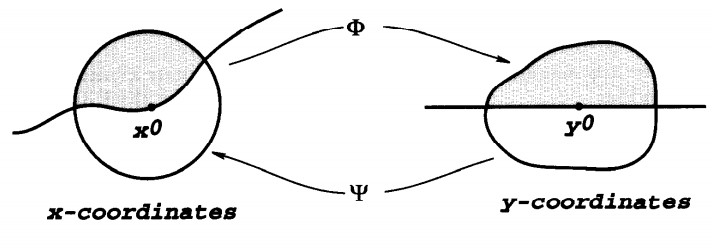
\includegraphics[scale=.35]{flatb}
\caption{\tiny{L. C. Evans, \textit{Partial Differential Equations}}}
\end{figure}
\end{frame}

\begin{frame}
\begin{enumerate}
\item Selezioniamo una variabile privilegiata e chiamiamola ``tempo'':
\begin{align*}
t & \leftarrow x_n \\
x & \leftarrow (x_1,\ldots , x_{n-1})
\end{align*}
\item Chiamiamo $\Gamma = \{t=0\}$.
\item Indichiamo le derivate nel modo seguente: $D^j_t D^\alpha_x u$.
\item Otteniamo il problema ($u^*=u(\Phi)$):
\begin{equation*}
\begin{cases}
F(x,t, D^j_t D^\alpha_x u)=0 & |\alpha | +j \leq k\\
D^j_t u (x,0)= \phi_j(x) & \text{per }j<k 
\end{cases}
\end{equation*}
\end{enumerate}
\end{frame}

\begin{frame}
\frametitle{Superfici non caratteristiche in generale}
\begin{definition}
$\Gamma^*$ (o $\Gamma$) è non caratteristica $\iff$ l'equazione su $\Gamma$ può essere riscritta in \textbf{forma normale} rispetto a $t$.
\end{definition}
\begin{remark}
Si dimostra che è coerente con le definizioni precedenti.
\end{remark}
\begin{remark}
\begin{itemize}
\item Caso lineare $\rightarrow$ condizione sui coefficienti.
\item Caso non lineare $\rightarrow$ validità ipotesi teorema del Dini su $F$.
\end{itemize}
\end{remark}
\end{frame}


\begin{frame}
\frametitle{Serie di potenze notevole}
\begin{definition}
Funzione maggiorante: $$\mathcal{M}_{Cr}(x)=\frac{Cr}{r-(x_1+\ldots +x_n)}$$
\end{definition}
\begin{remark}
Per il teorema multinomiale se $|x|<r/n$ si ha che
$$\frac{Cr}{r-(x_1+\ldots +x_n)}=C \sum\limits_\alpha \frac{|\alpha |!}{\alpha ! \, r^{|\alpha |}} x^\alpha.$$
\end{remark}
\end{frame}

\begin{frame}
\frametitle{Metodo dei maggioranti}
\begin{theorem}[utilità del maggiorante]
\begin{equation*}
\begin{cases}
g_\alpha \geq |f_\alpha|\\
\sum g_\alpha x^\alpha \text{ ha raggio di conv. } R
\end{cases}
\implies 
\begin{array}{c}
\sum f_\alpha x^\alpha \\
\text{ha raggio almeno } R
\end{array}
\end{equation*}
\end{theorem}
In questo caso si scrive:  $\sum g_\alpha x^\alpha \gg \sum f_\alpha x^\alpha$.
\end{frame}

\begin{frame}
\begin{theorem}[costruzione del maggiorante]
$\sum f_\alpha x^\alpha$ ha raggio $R \implies \exists \, r<R, \, C>0$ tali che 
$$|f_\alpha | \leq C \frac{1}{r^{|\alpha |}} \leq C \frac{|\alpha |!}{\alpha ! \, r^{|\alpha |}}$$
\end{theorem}
\end{frame}


\section{Versione invariante}


\begin{frame}
\frametitle{Schema dell'approccio}
Seguendo l'ordine cronologico di scoperta procediamo per \textbf{generalizzazioni progressive}:
\begin{enumerate}
\item EDO
\item EDP quasi-lineari
\item EDP in forma normale
\end{enumerate}
\end{frame}


\begin{frame}
\frametitle{EDO}
Teorema di unicità $f:A\times B\rightarrow\mathbb{C}^n$ olomorfa (A, B aperti)
\begin{equation}
\begin{system}
y' = f(x,y) \quad \forall x \in \Omega \\
y(x_0)=y_0
\end{system}
\end{equation}
Se la soluzione esiste è unica
\end{frame}

\begin{frame}
Teorema di esistenza locale con stima del raggio
\end{frame}

\begin{frame}
\frametitle{EDP quasi-lineari}
Forma particolare del sistema di interesse
\end{frame}

\begin{frame}
DIMOSTRAZIONE: metodo delle caratteristiche e metodo dei maggioranti
\begin{enumerate}
\item si osserva come i coefficienti di una serie di potenze che risolve l'equazione devono essere dei polinomi a coefficienti non negativi
\item $A_i^* \gg A_i, B^* \gg B \implies u^* \gg u$
\item si scelgono $A_i^*, B^*$ in modo tale da poter calcolare esplicitamente una soluzione analitica con il metodo delle caratteristiche
\end{enumerate}
\end{frame}

\begin{frame}
\frametitle{Stima del raggio di convergenza}
Ricordando la stima:
$$\widetilde{r} = \dfrac{1}{n-1}\, \dfrac{r}{8Cmn} \text{ con } C \geq \frac{1}{2}$$
Osserviamone l'andamento rispetto a $r$, sapendo che:
\begin{align*}
r <& \min \{ \textit{raggi di conv. dei coefficienti } a^i_{ml}, \, b_m\} \\
C \geq & \max \begin{Bmatrix}
\max\limits_{i,m,l,\alpha } \left|a^i_{ml} \, r^{|\alpha |}\right|\\
\max\limits_{m,\alpha} \left|b_m \, r^{|\alpha |}\right|
\end{Bmatrix}
\end{align*}
\end{frame}

\begin{frame}
\frametitle{EDP non lineari}
Forma particolare del sistema di interesse
\end{frame}

\begin{frame}
\frametitle{EDP non lineari}
Trasformazione nel sistema quasi-lineare precedente (che è il grande merito di Kowalevski)
\end{frame}




\section{Esempi}

\begin{frame}
\frametitle{Esempio di Lewy}
Importanza della richiesta di analiticità
\end{frame}

\begin{frame}
generalizzazione esempio di Lewy, enunciato
\begin{theorem}
\hpth{
A \subseteq \mathbb{R}^3 \text{ aperto }\\
}
{
\exists \, F \in C^{\infty}(\mathbb{R}^3,\mathbb{R}) \; : \; \nexists \, u \in C^1(A,\mathbb{R}) \\ \text{ tale che }
\begin{system}
Lu=F \text{ in } A\\
\vspace{-2mm}
u_x,\,u_y,\,u_t \text{ soddisfano} \\
\text {la condizione di Hölder }
\end{system}
}
\end{theorem}
\end{frame}

\begin{frame}
Idea della dimostrazione:
\begin{enumerate}
\item
traslare il problema del teorema precedente in modo da ricondursi al caso di un generico punto $(x_0,y_0,t_0)$, usando come forzante la funzione $g(x,y,t)=f(t-2xy_0+2x_0y)$;
\item
costruire con una serie una funzione $S_a \in C^\infty$ per ogni $a \in l^\infty$;
\item
costruire degli insiemi $E_{j,n} \subseteq l^\infty$ chiusi e senza parte interna sfruttando $S_a$ e il teorema di Ascoli-Arzelà;
\item
concludere la dimostrazione del nuovo teorema utilizzando i lemmi appena citati per ricavare, con un ragionamento per assurdo, l'uguaglianza $l^\infty = \bigcup E_{j,n}$, grazie alla quale si può applicare l'argomento di Baire.
\end{enumerate}
\end{frame}

\begin{frame}
\frametitle{Esempio di Kowalevski}
Importanza superfici non caratteristiche
\end{frame}

\begin{frame}
\frametitle{Esempio di Hadamard}
Nessuna garanzia della stabilità della soluzione
\end{frame}



\section{Versioni alternative}

\begin{frame}
\frametitle{Versione classica}
Enunciato, può essere visto come corollario di un teorema più astratto.
\end{frame}

\begin{frame}
\frametitle{Versione astratta}
Premessa $$E_s = H(\overline{\mathcal{O}_s}; \mathbb{C}^m)$$ con $s \in [0,1]$, costante $C$
\end{frame}

\begin{frame}
Enunciato
\end{frame}

\begin{frame}
Dimostrazione esistenza
\end{frame}

\begin{frame}
Dimostrazione unicità
\end{frame}

\begin{frame}
\frametitle{Versioni "olomorfe"}
Si può rifare tutto con $t$ variabile complessa e i teoremi non cambiano. Lo stesso vale anche per la versione invariante normale.
\end{frame}




\section{Applicazioni}

\begin{frame}
Le conseguenze di questo teorema si osservano in vari campi, tra cui i principali sono:
\begin{itemize}
\item teoria delle equazioni differenziali
\item fisica matematica: emersione di numerose domande (cosa succede nella realtà se esiste una sol. analitica locale?)
\item geometria differenziale
\item teoria economica
\end{itemize}
\end{frame}

\begin{frame}
Impatto sulla teoria delle equazioni differenziali:
\begin{itemize}
\item confutare la congettura di Weierstrass (ogni funzione è 
\item teorema di Holmgren
\item Treves e Nierenberg per la ricerca di condizioni necessarie e/o sufficienti per l'esistenza di soluzioni locali
\item Hormander la teoria degli operatori differenziali lineari (con particolare attenzione alla condizioni necessarie)
\end{itemize}
\end{frame}

\begin{frame}
\frametitle{Teorema di Holmgren}
Enunciato astratto, si dimostra utilizzando la versione astratta di CK
\end{frame}


\begin{frame}
Enunciato concreto
\end{frame}

\begin{frame}
Sketch della dimostrazione
\end{frame}

\begin{frame}
\frametitle{Teorema di Cartan-Kähler}
Per quanto riguarda geometria differenziale e teoria economica abbiamo un risultato che seguire dal teorema di CK

Enunciato e applicazione al campo economico
\end{frame}

\begin{frame}
Nonostante la ricerca condotta in quegli anni
\begin{itemize}
\item non fosse guidata da applicazioni immediate
\item portò a risultati deludenti rispetto alle aspettative di Cauchy e Weierstrass
\end{itemize}
ha avuto un impatto gigantesco grazie alla comprensione delle soluzioni di sistemi di EDP che ci ha permesso di raggiungere.
\end{frame}

\begin{frame}

\begin{center}
\textit{
Era una vita -- gli costava dirlo, come ebbe ad ammettere,
perché si era sempre guardato dagli eccessivi entusiasmi --, era una vita
che aspettava di veder entrare nel suo studio un allievo del genere. 
Un allievo in grado di lanciargli una sfida assoluta, 
di non seguire soltanto il percorso spericolato della sua mente, 
ma se possibile di spiccare un volo più alto.
}
\end{center}
\null\hfill --- Alice Munro, \textit{Too Much Happiness}
\end{frame}

\end{document}
